\documentclass[10pt,a4paper]{article}
\usepackage[utf8]{inputenc}
\usepackage[italian]{babel}
\usepackage{amsmath}
\usepackage{amsfonts}
\usepackage{amssymb}
\usepackage{graphicx}
\usepackage[left=2cm,right=2cm,top=2cm,bottom=2cm]{geometry}

\author{Gruppo 1G.BT \\ Lorenzo Cavuoti, Francesco Sacco}
\title{Es02B: Circuito RC - Filtri passivi}
\begin{document}
\maketitle

\newcommand{\Vin}{\frac{1}{j\omega C}}

\section{Filtro passa basso}
\subsection{}
Usando il multimetro digitale abbiamo misurato il valore di $R1=3.29\pm 0.03 k\Omega$
e il valore di $C1=9.9\pm 0.4 nF$, la frequenza di taglio teorica risulta quindi
$F_{Tteorica}=4.9\pm 0.2$ con errore dominato dall'incertezza sulla misura della
capacità del condensatore. Sempre dalla teoria sappiamo che il guadagno è dato da
\begin{equation}
	A_f = \frac{1}{\sqrt{1+(f/f_T)^2}}
\end{equation}
Per $f\approx0$ $A_f\approx1$, ovvero a bassa frequenza il filtro non attenua 	il segnale, per $f=2kHz \quad A_{Vteorica}=0.93\pm0.02$ invece per $f=20kHz \quad A_{Vteorica}=0.238\pm0.006$
\subsection{}
Dalla misura con l'oscilloscopio risulta $A_V(2kHz)_{mis} = 0.92\pm0.05$ e $A_V(20kHz)_{mis} = 0.241\pm0.013$ entrambi compatibili entro una barra di errore dalla misura teorica.\\La frequenza di taglio misurata vedendo la frequenza a -3dB risulta $f_{Tmis}=4.83\pm0.06kHz$ con errore dominato dall'incertezza sulla scelta della frequenza, invece quella facendo il fit(absoute-sigma=False) risulta $f_{Tfit}=4.90\pm0.09kHz$. Anche in questi ultimi due casi il risultato è compatibile con il valore teorico atteso.
\begin{table}[h]
	\centering
	\begin{tabular}{ccccccc}
		\hline
f[Hz]&$V_{in}[V]$&$\sigma[V]$&$V_{out}[V]$&$\sigma[V]$&$A_V$&$\sigma$\\
		\hline
		\hline
56& 12.5& 0.5& 12.4& 0.5& 0.99& 0.06\\
100& 12.5& 0.5& 12.5& 0.5& 1.00& 0.06\\
194& 12.5& 0.5& 12.5& 0.5& 1.00& 0.06\\
467& 12.5& 0.5& 12.4& 0.5& 0.99& 0.06\\
2.08 k& 12.5& 0.5& 11.7& 0.5& 0.94& 0.06\\
4.85 k& 12.5& 0.5& 8.9& 0.4& 0.71& 0.04\\
8.56 k& 12.5& 0.5& 6.2& 0.3& 0.50& 0.03\\
20.0 k& 12.5& 0.5& 3.01& 0.13& 0.241& 0.015\\
22.5 k& 12.5& 0.5& 2.68& 0.11& 0.214& 0.012\\
76.1 k& 12.5& 0.5& 0.80& 0.04& $64\times 10^{-3}$& $4\times 10^{-3}$\\
96.4 k& 12.5& 0.5& 0.63& 0.03& $50\times 10^{-3}$& $3\times 10^{-3}$\\
294 k& 12.5& 0.5& 0.21& 0.01& $16.7\times 10^{-3}$& $0.9\times 10^{-3}$\\
1.07 M& 12.5& 0.5& $55\times 10^{-3}$ & $2\times 10^{-3}$& $4.4\times 10^{-3}$& $0.3\times 10^{-3}$\\
	\end{tabular}
	\caption{Valori di tensione in entrata e in uscita in funzione della frequenza misurati per il filtro passa basso}
\end{table}
\begin{figure}
	\centering
	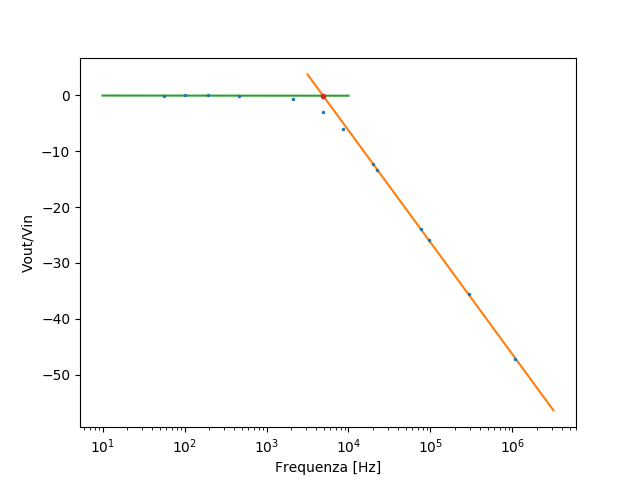
\includegraphics[scale=0.7]{a.png} 
	\caption{Plot di Bode passa basso}
\end{figure}
\subsection{}
La frequenza di taglio misurata dal gradino, ovvero dalla misura del tempo che impiega il segnale a passare dal 10\% al 90\% del massimo risulta $f_{Tgradino}=4.73\pm0.12kHz$. Il valore è ancora compatibile con la $F_T$ attesa, tuttavia è quello che si discosta di più rispetto alle altre misure.
\subsection{}
a) L'impedenza d'ingresso risulta
\begin{equation}
	Z_{in} = R+\frac{1}{j \omega C} = R(1-j\frac{\omega_T}{\omega})
\end{equation}
Quindi se
\begin{itemize}
\item $\omega>>\omega_T$ $|Z_{in}|=R$
\item $\omega=\omega_T$ $|Z_{in}|=\sqrt{2R}$
\item $\omega<<\omega_T$ $|Z_{in}|\rightarrow \infty$
\end{itemize}
b)
Se si inserisce una resistenza di carico il guadagno risulta
\begin{equation}
	A(\omega)=\frac{1}{\sqrt{(1+R/R_c)^2+(\omega RC)^2}}
\end{equation}
Ponendo l'espressione sopra uguale a $1/\sqrt{2}$ si può ottere una nuova frequenza di taglio
\begin{equation}
	\omega_t^2=\bigg[2-\bigg(1+\frac{R}{R_c}\bigg)^2\bigg]\frac{1}{(RC)^2}
\end{equation}
Quindi per $R_c=100k \omega$ abbiamo che $R_c>>R$ e le espressioni sopra si semplificano al circuito passa basso, invece per $R_c=10k \omega$ non si può trascurare $R_c$ $R_c\sim R$, di conseguenza alle stesse frequenze il guadagno risulta minore e in particolare si ha una diminuzione di $\omega_t$

\section{Filtro passa banda}
\subsection{Filtro RC passa alto}
Per il filtro passa alto abbiamo $R2=3.30\pm 0.03 k$ $C2=112\pm 5 nF$, la frequenza di taglio risulta quindi $F_{Tteorica}=430\pm20$, mentre con la misura all'oscilloscopio otteniamo $F_{Tmis}=450\pm10$, con errore dato dall'incertezza sulla scelta della frequenza, considerando gli errori i due risultati sono compatibili.
\subsection{Filtro passa banda}
a) $A_{0mis}=0.48\pm0.03$ $f_{Lmis}=215\pm7 Hz$ $f_{Hmis}=10.2\pm0.2 kH$, l'errore su $A_0$ è stato fatto propagando l'errore sul rapporto tra il segnale massimo in uscita e il segnale di ingresso, considerando i due errori scorrelati. L'errore sulle frequenze è stato determinato variando la frequenza di $V_{in}$ in modo da apprezzare sull’oscilloscopio una variazione di ampiezza di $V_out$\\
b) Per $f<<f_L$ aumentando la frequenza si osserva un aumento del guadagno, pari a circa 20dB/decade, per f compresa tra circa $2f_L$ e $f_H/2$ il guadagno è costante, pari a circa 0.48, infine per $f>>f_H$ si ha una diminuzione di ampiezza all'aumentare della frequenza pari a circa -20dB/decade. Il comportamento osservato è compatibile con la teoria, infatti per frequenze basse domina il passa alto, per frequenze alte invece domina il passa basso, in mezzo entrambi i filtri attenuano il segnale che risulta quindi costante.\\
c) Per far si che $V_{out}=A_1 A_2 V_{in}$ l'impedenza di ingresso del passa alto deve essere molto maggiore dell'impedenza di uscita del passa basso, quindi si deve avere che $R_2>>R_1$
\end{document}